% Copyright (c) Patrick Hall (jphall@gwu.edu), 2026--27. CC BY-NC-SA 4.0.
\documentclass[aspectratio=169]{beamer}
\usetheme{Singapore}
\definecolor{brand}{RGB}{45,110,191}
\definecolor{hrgray}{RGB}{100,100,100}
\definecolor{safe}{RGB}{37,125,83}
\definecolor{warn}{RGB}{180,105,0}
\setbeamercolor{structure}{fg=brand}
\setbeamercolor{title}{fg=hrgray}
\setbeamercolor{subtitle}{fg=brand}
\setbeamercolor{frametitle}{fg=hrgray}
\setbeamercolor{block title}{fg=white,bg=brand}
\setbeamercolor{block body}{bg=black!2}
\usepackage[T1]{fontenc}
\usepackage[utf8]{inputenc}
\usepackage{lmodern,microtype,graphicx,booktabs,tikz,amsmath,listings,array}
\usepackage[backend=biber,style=authoryear,maxcitenames=2,maxbibnames=10,doi=false,isbn=false]{biblatex}
\addbibresource{references.bib}
\DeclareBibliographyCategory{referencesone}
\DeclareBibliographyCategory{referencestwo}
\addtocategory{referencesone}{OpenAI2026Responses,OpenAI2026StructuredOutputs,OpenAI2026RateLimits,OpenAI2026ErrorCodes,JsonSchema2022,Bray2017JSON,Pydantic2026}
\addtocategory{referencestwo}{Guo2017Calibration,NIST2024GenAIProfile}
\renewcommand*{\mkbibacro}[1]{#1}
\renewcommand*{\bibfont}{\scriptsize}
\usetikzlibrary{positioning,arrows.meta,shapes.geometric}
\setbeamertemplate{navigation symbols}{}
\setbeamertemplate{bibliography item}{}
\setbeamertemplate{frametitle continuation}{}
\setbeamertemplate{footline}{\leavevmode\hbox{\begin{beamercolorbox}[wd=.5\paperwidth,ht=3ex,dp=1ex,left]{author in head/foot}\hspace{0.8ex}
\includegraphics[height=.5cm]{../../asset/gw_logo.png}\end{beamercolorbox}\begin{beamercolorbox}[wd=.5\paperwidth,ht=3ex,dp=1ex,right]{date in head/foot}\insertframenumber/\inserttotalframenumber\hspace{2ex}\end{beamercolorbox}}}
\title{Lecture 3: Model APIs, structured outputs, and typed decisions}
\author[Patrick Hall]{\textbf{Patrick Hall}}
\institute{Department of Decision Sciences}
\date{\today}
\newcommand{\slidesource}[1]{\vfill{\raggedright\tiny\color{hrgray}Source: #1\par}}
\newcommand{\visualdescription}[1]{\par\vspace{.2em}{\centering\tiny\color{hrgray}#1\par}}
\lstset{language=Python,basicstyle=\ttfamily\tiny,keywordstyle=\color{brand}\bfseries,stringstyle=\color{safe},commentstyle=\color{hrgray}\itshape,showstringspaces=false,columns=fullflexible,breaklines=true}
\begin{document}

\begin{frame}
  \titlepage
  \vspace{-.75em}
  \centering\scriptsize \textcopyright\ 2026--27 Patrick Hall (jphall@gwu.edu). Some rights reserved. Text and copy are licensed under a \href{https://creativecommons.org/licenses/by-nc-sa/4.0/}{Creative Commons Attribution-NonCommercial-ShareAlike 4.0 International License (CC BY-NC-SA 4.0)}.
  \begin{tikzpicture}[remember picture,overlay]
    \node[opacity=.08] at (current page.center) {
\includegraphics[width=.55\paperwidth]{../../asset/gw_logo.png}};
  \end{tikzpicture}
\end{frame}

\begin{frame}{Agenda}\tableofcontents\end{frame}

\section[API Requests]{API Requests and Parameters}
\begin{frame}{An API call is a bounded application transaction}
\footnotesize
\begin{center}
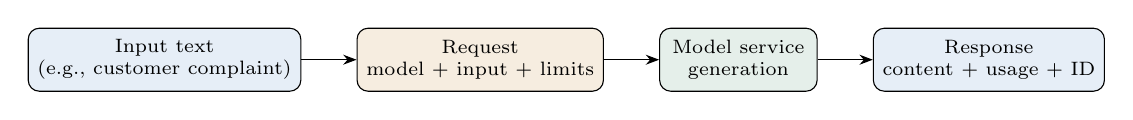
\begin{tikzpicture}[node distance=.6cm and .7cm, every node/.style={align=center,font=\scriptsize}]
\node[draw,rounded corners,fill=brand!12,minimum width=2cm,minimum height=.8cm] (app) {Input text\\(e.g., customer complaint)};
\node[draw,rounded corners,fill=warn!12,right=of app,minimum width=2cm,minimum height=.8cm] (request) {Request\\model + input + limits};
\node[draw,rounded corners,fill=safe!12,right=of request,minimum width=2cm,minimum height=.8cm] (service) {Model service\\generation};
\node[draw,rounded corners,fill=brand!12,right=of service,minimum width=2cm,minimum height=.8cm] (response) {Response\\content + usage + ID};
\draw[-{Stealth}] (app)--(request); \draw[-{Stealth}] (request)--(service); \draw[-{Stealth}] (service)--(response);
\end{tikzpicture}
\visualdescription{A four-stage path separates the application’s input and constraints from the model service’s response and operational metadata.}
\end{center}
\begin{itemize}
  \item A request chooses a model, supplies input and operating limits, and may attach response-format constraints.
  \item Preserve the request ID, model, completion state, usage, and application version for diagnosis and accounting; take care when logging sensitive text.
  \item Keep credentials out of source code: load \texttt{OPENAI\_API\_KEY} from an ignored \texttt{.env} file or obtain it interactively.
\end{itemize}
\slidesource{Responses API fields and lifecycle: \textcite{OpenAI2026Responses}.}
\end{frame}

\begin{frame}[fragile]{Inspect the response, not only its visible text}
\small
\begin{columns}[T]
\column{.51\textwidth}
{\lstset{basicstyle=\ttfamily\scriptsize}
\begin{lstlisting}
response = client.responses.create(
    model="gpt-5-mini",
    input="Customer says: charged twice...",
    max_output_tokens=250,
)
print(response.output_text)
print(response.id)
print(response.status)
print(response.usage)
\end{lstlisting}
}
\par\vspace{.2em}{\raggedright\tiny\color{hrgray}Python code prints both the visible answer and the operational fields needed to observe one API call.\par}
\column{.44\textwidth}
\begin{block}{Illustrative inspection}
\ttfamily\tiny
id: resp\_...\newline
status: completed\newline
input\_tokens: 46\newline
output\_tokens: 91\newline
visible text: ``I am sorry \ldots''
\end{block}
The generated text may be most interesting to the user, but the ID, status, and usage help an application decide what to retain, retry, charge, or investigate.
\end{columns}
\slidesource{Response objects and usage fields: \textcite{OpenAI2026Responses}.}
\end{frame}

\begin{frame}{Parameters are part of the operating contract}
\scriptsize
\begin{center}
{\setlength{\tabcolsep}{3pt}\renewcommand{\arraystretch}{1.18}
\begin{tabular}{>{\raggedright\arraybackslash}p{.17\linewidth}>{\raggedright\arraybackslash}p{.22\linewidth}>{\raggedright\arraybackslash}p{.28\linewidth}>{\raggedright\arraybackslash}p{.22\linewidth}}
\toprule
Control & Example value & Purpose & Application question \\ \midrule
Model & \texttt{gpt-5-mini} & capability, price, context, and supported features & Is this model fit for the task? \\
Output limit & \texttt{800 tokens} & caps visible and internal generation budget & What is a useful maximum response? \\
Sampling & \texttt{temperature=0.2} & varies output diversity when supported & Is variation useful here? \\
Reasoning & \texttt{minimal} & allocates deliberation where supported & Is extra latency worth it? \\
Timeout / retry & \texttt{45 s; 3 tries} & bounds waiting and repeated work & When should the caller stop? \\
Rate / spend & \texttt{60 req/min; daily cap} & protects availability and budget & What occurs under pressure? \\ \bottomrule
\end{tabular}}
\end{center}
\visualdescription{Illustrative settings show how an application makes model behavior, resource use, and failure boundaries explicit.}
\vspace{3pt}
Settings and names differ across models and providers. Treat a request configuration as versioned application code, not as universal model behavior.
\vspace{4pt}
\slidesource{Model-specific request capabilities: \textcite{OpenAI2026Responses}; rate-limit concepts: \textcite{OpenAI2026RateLimits}.}
\end{frame}

\begin{frame}[fragile]{Compare configurations on the same complaint}
\small
\begin{columns}[T]
\column{.59\textwidth}
\begin{lstlisting}
import time

def run(label, **settings):
    started = time.perf_counter()
    response = client.responses.create(
        model="gpt-5-mini", input=COMPLAINT,
        max_output_tokens=250, **settings,
    )
    return {
        "label": label, "seconds": time.perf_counter() - started,
        "tokens": response.usage.output_tokens,
        "text": response.output_text,
    }

fast = run("bounded", reasoning={"effort": "minimal"})
careful = run("deliberate", reasoning={"effort": "medium"})
\end{lstlisting}
\par\vspace{.2em}{\raggedright\tiny\color{hrgray}A small experiment holds the complaint and output cap constant while changing one supported setting and records time, tokens, and text.\par}
\column{.37\textwidth}
\begin{block}{Illustrative results}
\ttfamily\tiny
bounded\\
1.2 s; 74 output tokens\\
"I am sorry about the duplicate charge \ldots"\\[.45em]
deliberate\\
2.9 s; 112 output tokens\\
"The duplicate charge appears to be \ldots"
\end{block}
\small
Both answers may be usable. The deliberate setting used more time and tokens, so retain it only if evaluation shows enough added value for the task.
\end{columns}
\slidesource{Reasoning and output controls are model-dependent: \textcite{OpenAI2026Responses}.}
\end{frame}

\begin{frame}[fragile]{Streaming improves interaction; it does not change validation}
\footnotesize
\begin{columns}[T]
\column{.57\textwidth}
\begin{lstlisting}
stream = client.responses.create(
    model="gpt-5-mini",
    input="Acknowledge this complaint.",
    stream=True,
)
parts = []
for event in stream:
    if event.type == "response.output_text.delta":
        parts.append(event.delta)
        print(event.delta, end="", flush=True)
final_text = "".join(parts)
\end{lstlisting}
\column{.38\textwidth}
\begin{block}{Illustrative stream}
\ttfamily\tiny
[3 s elapsed]\\
I am sorry about\\
the duplicate charge.\\[.5em]
[10 s elapsed]\\
I am sorry about the duplicate\\
charge. I will help investigate.\\[.5em]
final\_text\\
I am sorry about the duplicate\\
charge. I will help investigate.
\end{block}
\end{columns}
\visualdescription{A streaming loop makes text fragments available as they arrive while retaining the complete assembled text for the application.}
\begin{itemize}\small
  \item Stream prose when an early fragment improves the user experience.
  \item Buffer structured content until complete; then parse and validate it.
  \item Show a truthful working state; an incomplete stream is not a completed output.
\end{itemize}

\slidesource{Streaming response events: \textcite{OpenAI2026Responses}.}
\end{frame}

\begin{frame}{Failure is not one category}
\footnotesize
{\scriptsize
\begin{center}\begin{tabular}{>{\raggedright\arraybackslash}p{.25\linewidth}>{\raggedright\arraybackslash}p{.28\linewidth}>{\raggedright\arraybackslash}p{.33\linewidth}}
\toprule
Observed outcome & Meaning & Bounded handling \\ \midrule
Network timeout or 5xx & service outcome unknown & retry only work safe to repeat; use exponential backoff \\
429 rate limit & caller exceeded an allocation & honor \texttt{Retry-After}; queue or shed load \\
Refusal & model declined the task & route to a safe alternative or human review \\
Incomplete response & output stopped before completion & record status; retry or request a shorter result \\
Schema or Pydantic error & text/data fails the contract & do not execute; repair once or escalate \\
Business-rule error & valid shape, unacceptable decision & reject and review the policy or evidence \\ \bottomrule
\end{tabular}\end{center}
}
\visualdescription{Distinguish transport and rate-limit problems from refusals, incomplete work, structural errors, and business-rule violations.}
\vspace{3pt}
Retries are explicitly designed and bounded attempts, not an automatic infinite loop. Add a unique ID and log the class of failure without duplicating sensitive content.
\vspace{3pt}
\slidesource{Service error classes and rate limits: \textcite{OpenAI2026ErrorCodes}; \textcite{OpenAI2026RateLimits}.}
\end{frame}

\section[Schemas]{Schemas and data contracts}
\begin{frame}{JSON is syntax; a schema is a contract}
\footnotesize
\begin{columns}[T]
\column{.46\textwidth}
\begin{block}{Syntactically valid JSON}
\ttfamily\tiny \{"category": "billing", "refund": -25\}
\end{block}
It parses, but a negative refund may violate business meaning.
\column{.49\textwidth}
\begin{block}{Schema-constrained object}
\ttfamily\tiny
\{\newline
\hspace*{1em}"type": "object",\newline
\hspace*{1em}"required": ["category", "refund"],\newline
\hspace*{1em}"properties": \{\newline
\hspace*{2em}"category": \{\newline
\hspace*{3em}"enum": ["billing", "delivery"]\newline
\hspace*{2em}\},\newline
\hspace*{2em}"refund": \{\newline
\hspace*{3em}"type": "number", "minimum": 0\newline
\hspace*{2em}\}\newline
\hspace*{1em}\}\newline
\}
\end{block}
The schema specifies fields, types, required values, enumerations, and nested structure.
\end{columns}
\vspace{4pt}
\visualdescription{Two compact JSON examples contrast parsable data with a schema that adds required fields, allowed values, and a numeric range.}
\vspace{10pt}
Schema-constrained generation can improve format reliability, but it does not establish that a category or amount is substantively correct.
\vspace{4pt}
\slidesource{JSON syntax: \textcite{Bray2017JSON}; schema vocabulary: \textcite{JsonSchema2022}; constrained generation: \textcite{OpenAI2026StructuredOutputs}.}
\end{frame}

\begin{frame}[fragile]{Extract complaint facts into a constrained object}
\footnotesize
\begin{columns}[T]
\column{.52\textwidth}
{\lstset{basicstyle=\ttfamily\tiny}
\begin{lstlisting}
complaint_format = {
  "type": "json_schema",
  "name": "complaint_facts",
  "strict": True,
  "schema": {
    "type": "object",
    "additionalProperties": False,
    "required": ["category", "amount", "evidence"],
    "properties": {
      "category": {
        "type": "string",
        "enum": ["billing", "delivery", "access"]
      },
      "amount": {
        "type": ["number", "null"], "minimum": 0
      },
      "evidence": {
        "type": "string", "minLength": 10
      }
    }
  }
}
\end{lstlisting}
}
\column{.43\textwidth}
\begin{lstlisting}
response = client.responses.create(
    model="gpt-5-mini",
    input=COMPLAINT,
    text={"format": complaint_format},
)
payload = json.loads(
    response.output_text
)
\end{lstlisting}
\begin{block}{Example output}
\ttfamily\tiny
\{"category": "billing",\newline
\hspace*{.8em}"amount": 24.99,\newline
\hspace*{.8em}"evidence": "charged twice"\}
\end{block}
Schema constraints shape the payload; local Python checks it before use.
\end{columns}
\vspace{-8pt}
\visualdescription{The left column defines the data contract; the right column passes it to a Responses API call and reads the returned JSON.}
\vspace{3pt}
The \texttt{evidence} field anchors the result in complaint text. Compare it with the source before acting.
\vspace{4pt}
\slidesource{JSON Schema constraints: \textcite{JsonSchema2022}; provider-specific structured-output request format: \textcite{OpenAI2026StructuredOutputs}.}
\end{frame}

\begin{frame}[fragile]{Pydantic turns a data contract into executable checks}
\footnotesize
\begin{columns}[T]
\column{.43\textwidth}
\begin{itemize}\scriptsize
  \item Pydantic is a Python library for parsing and validating data.
  \item Typed Python fields become runtime validation and JSON Schema.
  \item \texttt{model\_validate} returns a validated object or raises \texttt{ValidationError}.
  \item One schema can support request construction, response validation, and application-side checks.
  \item Alternatives include direct \texttt{jsonschema} checks, Marshmallow, or \texttt{dataclasses} with manual validation.
\end{itemize}
\column{.52\textwidth}
\begin{lstlisting}
from pydantic import BaseModel, Field, ValidationError

class RefundLookup(BaseModel):
    charge_id: str = Field(min_length=10)
    refund_amount: float = Field(ge=0)

try:
    args = RefundLookup.model_validate(payload)
except ValidationError as error:
    print(error.errors())  # inspect; do not use the payload
\end{lstlisting}
\par\vspace{.2em}{\raggedright\tiny\color{hrgray}The code defines a refund-request schema, then turns a payload into validated arguments or reports a validation error.\par}
\end{columns}
\slidesource{Pydantic models and generated JSON Schema: \textcite{Pydantic2026}; schema concepts: \textcite{JsonSchema2022}.}
\end{frame}

\begin{frame}[fragile]{Structural validation is necessary but not sufficient}
\footnotesize
\begin{columns}[T]
\column{.48\textwidth}
\begin{lstlisting}
class Refund(BaseModel):
    amount: float = Field(gt=0, le=250)
    currency: Literal["USD"]

class Triage(BaseModel):
    action: Literal["request_information",
                    "recommend_refund", "escalate"]
    rationale: str = Field(min_length=10)
    refund: Refund | None = None
\end{lstlisting}
\vfill
\begin{lstlisting}
def business_check(t: Triage):
    if t.action == "recommend_refund" and not t.refund:
        raise ValueError("refund is required")
    if t.action != "recommend_refund" and t.refund:
        raise ValueError("refund is not allowed")
\end{lstlisting}
\column{.47\textwidth}
\vspace{.3em}
\begin{block}{Business-rule inputs}
\scriptsize
\begin{tabular}{@{}l@{\qquad}l}
\textcolor{safe!70!black}{\textbf{Pass}} & \texttt{action: "recommend\_refund"} \\
& \texttt{refund: 24.99 USD} \\[.25em]
\textcolor{red!75!black}{\textbf{Fail}} & \texttt{action: "escalate"} \\
& \texttt{refund: 24.99 USD}
\end{tabular}
\end{block}
\end{columns}
\visualdescription{A typed triage record and a second business-rule function enforce that a refund exists only for the refund recommendation.}
\begin{itemize}\scriptsize
  \setlength{\itemsep}{.2em}
  \item Field relationships are business rules; state them explicitly.
  \item The same parsed input always gives the same accept-or-reject result.
  \item Run this deterministic, application-side guardrail before acting---not as another model judgment.
\end{itemize}
\slidesource{Data-model validation: \textcite{Pydantic2026}; structural controls are one component of generative-AI risk management \parencite{NIST2024GenAIProfile}.}
\end{frame}

\begin{frame}[fragile]{Schemas also make tool boundaries inspectable}
\footnotesize
\begin{columns}[T]
\column{.55\textwidth}
\begin{center}
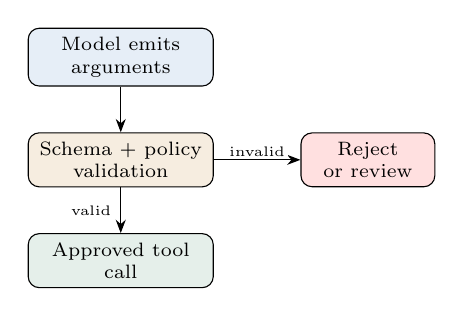
\begin{tikzpicture}[node distance=.58cm,every node/.style={font=\scriptsize,align=center}]
\node[draw,rounded corners,fill=brand!12,minimum width=2.35cm,minimum height=.65cm] (m) {Model emits\\arguments};
\node[draw,rounded corners,fill=warn!12,below=of m,minimum width=2.35cm,minimum height=.65cm] (v) {Schema + policy\\validation};
\node[draw,rounded corners,fill=safe!12,below=of v,minimum width=2.35cm,minimum height=.65cm] (t) {Approved tool\\call};
\node[draw,rounded corners,fill=red!12,right=1.1cm of v,minimum width=1.7cm,minimum height=.65cm] (h) {Reject\\or review};
\draw[-{Stealth}] (m)--(v);
\draw[-{Stealth}] (v)--node[left]{\tiny valid} (t);
\draw[-{Stealth}] (v)--node[above,fill=white,inner sep=1pt]{\tiny invalid} (h);
\end{tikzpicture}
\end{center}
\column{.4\textwidth}
\begin{block}{Illustrative pseudocode}
\begin{lstlisting}
valid = {"charge_id": "ch_482",
         "refund_amount": 24.99}
args = RefundLookup.model_validate(valid)
lookup_recent_charge(args.charge_id)  # tool
# accepted: {"status": "pending"}

invalid = {"charge_id": "ch_482",
           "refund_amount": -24.99}
# raises ValidationError: negative refund
RefundLookup.model_validate(invalid)
# no tool call; add to review queue
\end{lstlisting}
\end{block}
\end{columns}
\visualdescription{Validation routes model-produced arguments either to a tool call or to rejection and review.}
\vspace{5pt}
The application validates arguments before invocation; the model neither authorizes nor directly executes the lookup.
\slidesource{Structured outputs and function definitions: \textcite{OpenAI2026StructuredOutputs}; governance context: \textcite{NIST2024GenAIProfile}.}
\end{frame}

\section[Decisions]{Typed decisions}
\begin{frame}{A typed decision makes actions and uncertainty visible}
\footnotesize
\begin{center}\begin{tabular}{p{.25\linewidth}p{.28\linewidth}p{.29\linewidth}}
\toprule
Decision type & Required supporting fields & Example use \\ \midrule
\texttt{request\_information} & missing facts; one question & ``What date was the duplicate charge?'' \\
\texttt{recommend\_refund} & amount; currency; evidence & ``Refund \$24.99 for the duplicated charge.'' \\
\texttt{escalate} & reason; evidence; urgency & ``Possible fraud; specialist review required.'' \\ \bottomrule
\end{tabular}\end{center}
\visualdescription{A decision table gives each allowed triage action its own required evidence, amount, or question fields.}
\vspace{4pt}
This \href{https://jev-lab.com/en/guides}{\textcolor{brand}{Jev}}-style pattern treats a decision as a discriminated set of allowable alternatives, each with the information needed to act or review it. It prevents an ambiguous free-text answer from silently becoming an operational command.
\par\vspace{.2em}{\scriptsize Local option: \href{https://huggingface.co/h2oai/h2o-lightning-4b}{\textcolor{brand}{H2O-Lightning-4B}} is an open-weight, Apache-2.0 decision model that can run locally; validate it on your own cases.}
\vspace{4pt}
\slidesource{Practical decision-model guide: \href{https://jev-lab.com/en/guides}{TypeSafe AI, 2026, \emph{A practical guide to Jev}}; local option: \href{https://huggingface.co/h2oai/h2o-lightning-4b}{H2O.ai, 2026, \emph{H2O-Lightning-4B}}; implementation with Pydantic: \textcite{Pydantic2026}.}
\end{frame}

\begin{frame}[fragile]{Request a typed triage decision from the API}
\footnotesize
\begin{columns}[T]
\column{.61\textwidth}
\begin{lstlisting}
result = client.decisions.create(
    model="gpt-6-luna",
    input=(
        "Policy: refund duplicate charges; escalate disputed "
        "evidence. Record: two claimed charges; ledger has one."
    ),
    questions=[{
        "type": "choice", "name": "next_step",
        "instructions": "Select the next step.",
        "choices": [
            {"value": "refund", "description": "Recommend refund"},
            {"value": "abstain", "description": "Request more evidence"},
            {"value": "escalate", "description": "Request review"},
        ],
    }],
)
answer = result.answers[0]  # choice or refusal
\end{lstlisting}
\column{.34\textwidth}
\begin{block}{Choice answer}
\ttfamily\tiny
choice: "escalate"\newline
probabilities:\newline
\hspace*{.8em}refund:\hspace{1.2em}0.07\newline
\hspace*{.8em}abstain:\hspace{.6em}0.03\newline
\hspace*{.8em}escalate:\hspace{.3em}0.90\newline
confidence:\hspace{.2em}0.88
\end{block}
\end{columns}
\visualdescription{The API selects one supplied option and returns its confidence alongside probabilities for every allowed option.}
\begin{itemize}\scriptsize
  \setlength{\itemsep}{.1em}
  \item Only supplied next-step values can be returned; application code maps the choice to a local workflow.
  \item A choice answer includes all option probabilities and a confidence value.
  \item Reported probabilities are model scores, not calibrated guarantees.\parencite{Guo2017Calibration}
  \item Compare performance and cost to traditional statistical/ML classifiers. 
\end{itemize}
\vspace{2pt}
\slidesource{Decisions API, choice answers, probabilities, and confidence: \textcite{OpenAI2026Decisions}; calibration: \textcite{Guo2017Calibration}.}
\end{frame}

\begin{frame}{Abstention and escalation are decision outcomes}
\footnotesize
\begin{columns}[c]
\column{.48\textwidth}
\begin{block}{Complaint}
``I was charged twice, and someone changed the shipping address. I need this fixed today.''
\end{block}
\column{.47\textwidth}
\begin{block}{Typed result}
\ttfamily\tiny
\{"action":"escalate",\newline
"reason":"possible account takeover",\newline
"urgency":"high",\newline
"evidence":"shipping address changed"\}
\end{block}
\end{columns}
\visualdescription{A suspicious complaint maps to an escalation object with an explicit reason, urgency, and supporting text instead of an automated refund.}
\begin{itemize}\small
  \item \texttt{abstain} requests more evidence; \texttt{escalate} routes a risky or policy-sensitive case to a specialist.
  \item A returned choice guides the workflow; it does not authorize or execute an action.
  \item A deterministic application-side guardrail can override any returned choice and route the case to review.
\end{itemize}
\slidesource{Decision outcomes and choice answers: \textcite{OpenAI2026Decisions}.}
\end{frame}

\begin{frame}{Evaluate three different claims}
\footnotesize
\begin{center}\begin{tabular}{p{.25\linewidth}p{.30\linewidth}p{.28\linewidth}}
\toprule
Claim & Check & Example metric \\ \midrule
Structural validity & Does output parse and satisfy the contract? & schema-valid rate \\
Business-rule compliance & Does the object obey policy relationships? & invalid-action rate \\
Substantive correctness & Is the extraction or decision right for this case? & labeled extraction / decision accuracy \\
Escalation behavior & Does it defer when it should? & escalation precision and recall \\ \bottomrule
\end{tabular}\end{center}
\visualdescription{Decision evaluation should address output format, policy compliance, factual decision quality, and escalation behavior.}
\begin{itemize}\small
  \item A schema-valid decision can still be wrong.
  \item Keep a labeled, representative holdout set with routine, ambiguous, high-risk, and missing-information cases.
  \item Lecture 7 contains a fuller treatment of test, evaluation, verification, and validation (TEVV).
\end{itemize}
\vspace{4pt}
\slidesource{Evaluation should support a stated decision and risk context: \textcite{NIST2024GenAIProfile}.}
\end{frame}

\section{Synthesis}
\begin{frame}{A reliable model API application has layered controls}
\footnotesize
\begin{center}
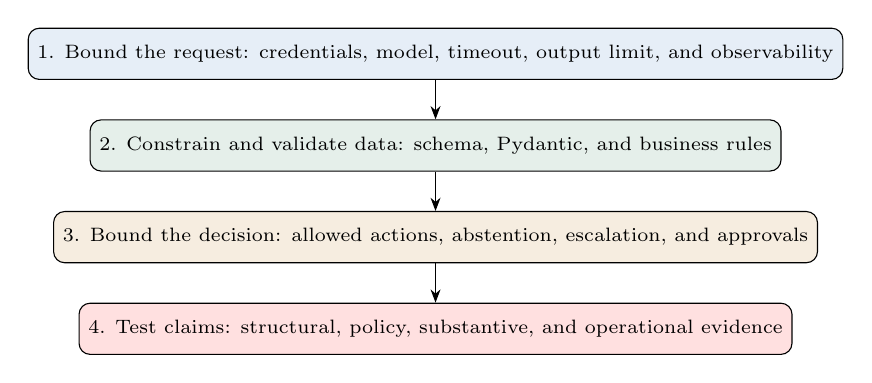
\begin{tikzpicture}[node distance=.5cm,every node/.style={font=\scriptsize,align=center,minimum height=.65cm}]
\node[draw,rounded corners,fill=brand!12,minimum width=8cm] (one) {1. Bound the request: credentials, model, timeout, output limit, and observability};
\node[draw,rounded corners,fill=safe!12,below=of one,minimum width=8cm] (two) {2. Constrain and validate data: schema, Pydantic, and business rules};
\node[draw,rounded corners,fill=warn!12,below=of two,minimum width=8cm] (three) {3. Bound the decision: allowed actions, abstention, escalation, and approvals};
\node[draw,rounded corners,fill=red!12,below=of three,minimum width=8cm] (four) {4. Test claims: structural, policy, substantive, and operational evidence};
\draw[-{Stealth}] (one)--(two); \draw[-{Stealth}] (two)--(three); \draw[-{Stealth}] (three)--(four);
\end{tikzpicture}
\end{center}
\visualdescription{Four stacked layers show the progression from bounded API requests to validated data, controlled decisions, and multi-level evaluation.}
\slidesource{API and structured-output behavior: \textcite{OpenAI2026Responses,OpenAI2026StructuredOutputs}; risk-management context: \textcite{NIST2024GenAIProfile}.}
\end{frame}

\section{References}
\begin{frame}[t]{References}\printbibliography[heading=none]\end{frame}
\end{document}
